\documentclass[12pt]{jarticle}
\usepackage{TUSIReport}
\usepackage{otf}
\usepackage[dvipdfmx]{graphicx}
\usepackage[dvipdfmx]{color}
\usepackage{amsmath}
\usepackage{amssymb}
\usepackage{color}
\usepackage{hhline}
\usepackage{fancybox,ascmac}
\usepackage{multirow}
\usepackage{url}
\usepackage{bm}
\usepackage{listings,jlisting}
\lstdefinestyle{log}{
    frame={tblr},
    basicstyle={\footnotesize},
    tabsize={4},
}
\lstdefinestyle{lstcpp}{
    language={c++},
    backgroundcolor={\color[gray]{.85}},
    basicstyle={\small},
    identifierstyle={\small},
    commentstyle={\small\ttfamily \color[rgb]{0,0.5,0}},
    keywordstyle={\small\bfseries \color[rgb]{1,0,0}},
    ndkeywordstyle={\small},
    stringstyle={\small\ttfamily \color[rgb]{0,0,1}},
    frame={tb},
    breaklines=true,
    columns=[l]{fullflexible},
    numbers=left,
    xrightmargin=0zw,
    xleftmargin=3zw,
    numberstyle={\scriptsize},
    stepnumber=1,
    numbersep=1zw,
    morecomment=[l]{//}
}
\begin{document}
%%%%%%%%%%%%%%%%%%%%%%%%%%%%%%%%%%%%%%%%%%%%%%%%%%%%%%%%%%%%%%
% 表紙を出力する場合は,\提出者と\共同実験者をいれる
% \提出者{科目名}{課題名}{提出年}{提出月}{提出日}{学籍番号}{氏名}
% \共同実験者{一人目}{二人目}{..}{..}{..}{..}{..}{八人目}
%%%%%%%%%%%%%%%%%%%%%%%%%%%%%%%%%%%%%%%%%%%%%%%%%%%%%%%%%%%%%%
\提出者{情報工学実験2}{実験テーマ3 情報通信シミュレーション}{2020}{12}{7}{4619055}{辰川力駆}
\共同実験者{}{}{}{}{}{}{}{}

%%%%%%%%%%%%%%%%%%%%%%%%%%%%%%%%%%%%%%%%%%%%%%%%%%%%%%%%%%%%%%
% 表紙を出力しない場合は,以下の「\表紙出力」をコメントアウトする
%%%%%%%%%%%%%%%%%%%%%%%%%%%%%%%%%%%%%%%%%%%%%%%%%%%%%%%%%%%%%%
\表紙出力

%%%%%%%%%%%%%%%%%%%%%%%%%%%%%%%%%%%%%%%%%%%%%%%%%%%%%%%%%%%%%%
% 以下はレポート本体である.別途 TeXファイルを作成し \input 使っても良い
%%%%%%%%%%%%%%%%%%%%%%%%%%%%%%%%%%%%%%%%%%%%%%%%%%%%%%%%%%%%%%

\section{実験概要}
 (7,4)ハミング符号による符号化、復号を行うプログラムを作成して、
ハミング符号の特徴を理解する。

\section{実験手順}
\begin{enumerate}
    \item 4ビットの情報 $\boldsymbol{w}$ を生成
    \item 生成多項式 $g(x)$ を用いて符号化
    \item 1ビットの雑音を付与する
    \item 受信語 $\boldsymbol{y}$ と検査行列 $H$ からシンドローム $\boldsymbol{s}$ を計算
    \item シンドロームから誤り位置を推定する
    \item 推定語 $\hat{\boldsymbol{x}}$ を求め、もとの $\boldsymbol{x}$ と値を比較する
\end{enumerate}

\section{実験結果}

ソースコードは付録に記述した。
$\epsilon=0.0001$として、SIMを1000000回実行した結果は上記のようになった。
また、それらの結果をグラフにプロットすると図1のようになった。
なお、縦軸は対数で表示している。

\begin{figure}[h]
    \begin{center}
        % 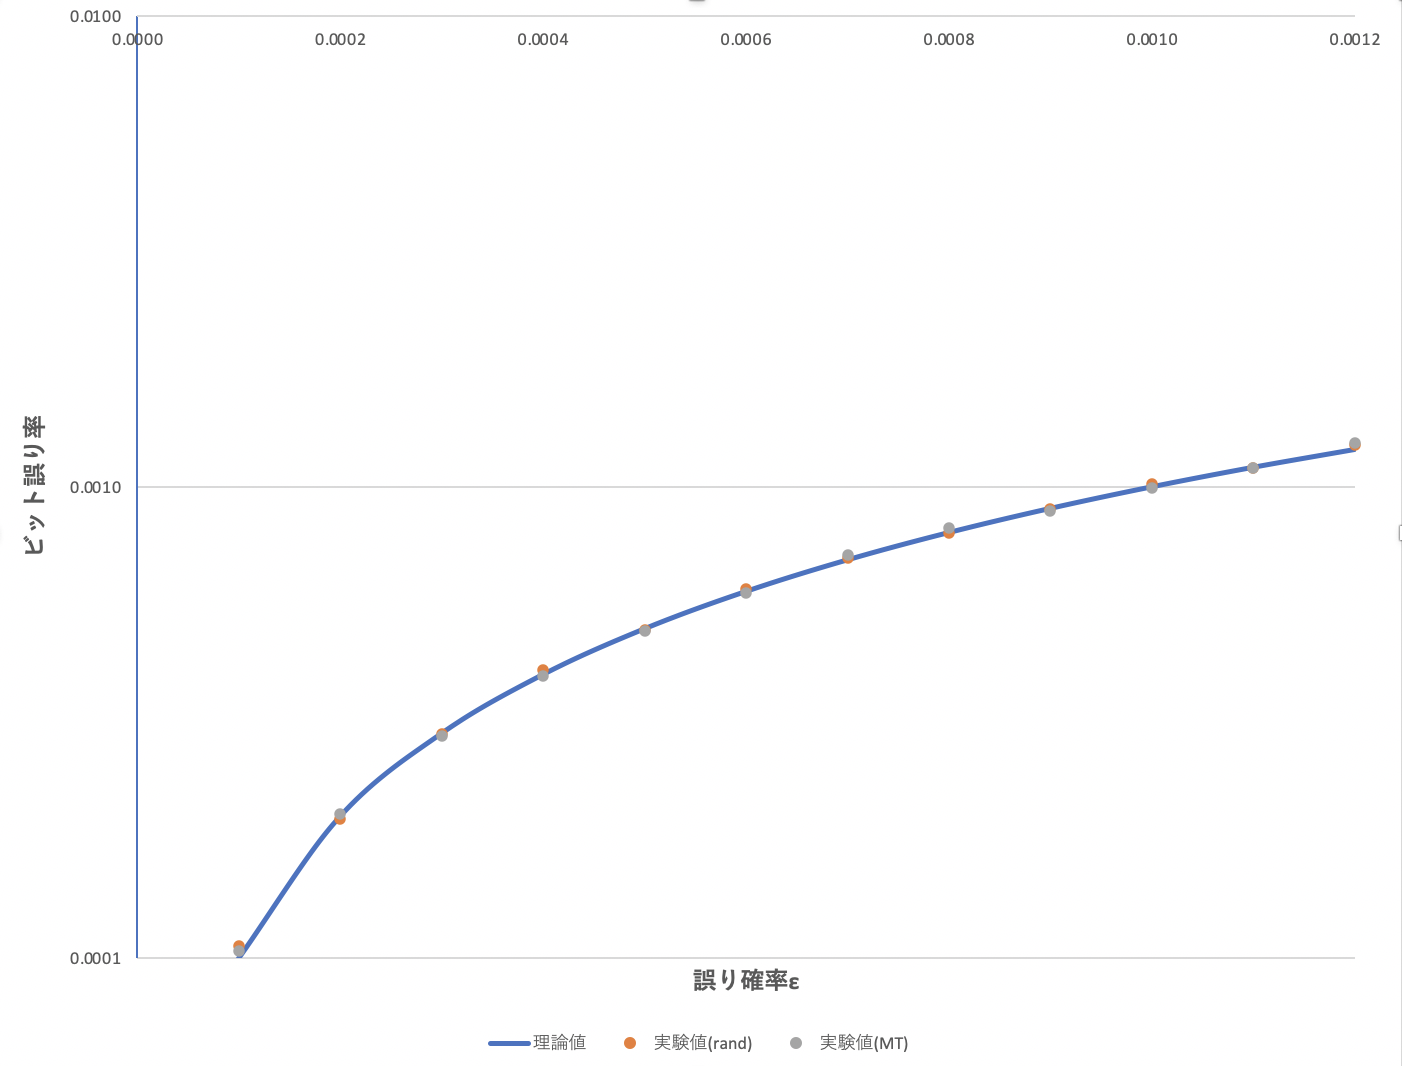
\includegraphics[scale=0.3]{kadai3_1_1.png}
    \end{center}
    \caption{ビット誤り率と誤り確率}
\end{figure}

\section{検討}
\subsection{課題1}
\begin{shadebox}
    シミュレーションによるビット誤り率と理論値が
    ほぼ同じ値になるにはどの程度のシミュレーション回数を実行する必要があるか。
\end{shadebox}

大数の法則より、シミュレーション回数を増やすほうが、
理論値に近づくのは明白である。
実際、SIM回数を1000000回から減らすと、
誤差が大きくなった。
さらに誤差を減らすためには1000000回以上行えばよいが、
実行するのに時間とてもかかってしまうだろう。

\subsection{課題2}
\begin{shadebox}
    $\epsilon$を非常に小さくした場合、これはどうなるか。
\end{shadebox}

$\epsilon$を実験よりさらに10分の1の値($\epsilon=0.00001$)とした場合、
以下のような結果となった。
行うことは同様であったが、誤差の割合を見ると大きくなっていると考えられる。
これは、理論値を小さくすることにより相対的に誤差の割合が大きくなっていると考えられる。


\clearpage

\subsection{課題3}
\begin{shadebox}
    $\rm{rand()}$と$\rm{MT}$の違いは何か。
\end{shadebox}

rand()関数は環境にもよるが$0\sim 32767$までの値しか取らない。
環境が違っていても少なくとも最大値が存在する。
今回は$0\sim 1$の値を求めるだけに使ったのであまり変わらなかったが、
$0\sim 10000$の値を求めるために乱数を使ったりするときは、
最大値が存在するから偏りが生じる。
よって、ほぼ均等に乱数を生成するならばメルセンヌ・ツイスタを用いるほうが良いと考える。

しかし、メルセンヌ・ツイスタで実行した場合、
実行速度が(rand()関数を用いた時より)遅くなるので、
速度を重視するか、性能を重視するかで使い分けると良いだろう。

\clearpage
% 付録
\appendix
\section{付録}
\begin{lstlisting}[style = lstcpp,caption=kadai3\_rand.cpp]
    //4619055 辰川力駆
    #include <random> // 乱数生成
    #include <stdio.h>
    #include <iostream>
    #include <iomanip>
    
    using namespace std;
    
    #define SIM 1000000
    
    #define real_rand (double)rand() / RAND_MAX; //RAND_MAXで割ることで0から1を返すようにしている。
    #define seed 55                              //学籍番号下2桁
    #define K 4                                  //系列長
    
    int main()
    {
        srand(seed);
        int w[4], e[4], y[4];
    
        cout << "# SIM:" << SIM << endl;
        cout << "# ep   # BER" << endl;
    
        double ep = 0;
        int count = 0;
        for (int i = 0; i < 12; i++) //12回で設定
        {
            count = 0;
            ep = 0.0001 * (i + 1);
    
            for (int s = 0; s < SIM; s++)
            {
                for (int j = 0; j < K; j++)
                {
                    double rd = real_rand; //乱数発生
                    w[j] = rd * 2;         //2倍することで0.5より大きいか小さいかを判定できる。
                }
                for (int j = 0; j < K; j++)
                {
                    double rd = real_rand; //乱数発生
                    if (rd <= ep)
                    {
                        e[j] = 1;
                    }
                    else
                    {
                        e[j] = 0;
                    }
                }
                for (int j = 0; j < K; j++)
                {
                    y[j] = w[j] ^ e[j];
                    count += w[j] ^ y[j];
                }
            }
            cout << fixed << setprecision(4) << ep;
            cout.unsetf(ios::fixed);
            cout << fixed << setprecision(7) << " " << (double)count / (K * SIM) << endl;
        }
    
        return 0;
    }
\end{lstlisting}

%%%%%%%%%%%%%%%%%%%%%%%%%%%%%%%%%%%%%%%%%%%%%%%%%%%%%%%%%%%%%%
\end{document}